\documentclass[12pt]{article}
\renewcommand{\thesection}{\Roman{section}} 
\renewcommand{\thesubsection}{\thesection.\Roman{subsection}}
%\usepackage[tocindentauto]{tocstyle}
%\usetocstyle{KOMAlike} %the previous line resets it
%\usepackage{natbib}
\usepackage{biblatex}
\addbibresource[]{ref.bib}
\usepackage{url}
\usepackage[utf8]{inputenc}
\usepackage{amsmath}
\usepackage{graphicx}
\usepackage{graphviz}
\usepackage[T1]{fontenc}
\graphicspath{{images/}}
\usepackage{parskip}
\usepackage{fancyhdr}
\usepackage{hyperref}
\usepackage{parskip}
\usepackage{hologo}
\usepackage{listings}
\usepackage{titlesec, blindtext, color}
\usepackage{titling}
\usepackage{tcolorbox}
\usepackage[hmargin=1in,vmargin=1in]{geometry}
\usepackage{float}
\usepackage{tikz}
\usepackage{appendix}
\usepackage{listings} % For code importing
\usepackage{xcolor} % for setting colors
\usepackage{svg}
\usepackage{tocloft}
\renewcommand{\cftsecleader}{\cftdotfill{\cftdotsep}}

\input{arduinoLanguage.tex}

\hypersetup{
	colorlinks=true,
	linkcolor=blue,
	urlcolor=cyan,
}

\lstdefinestyle{customc}{
  belowcaptionskip=1\baselineskip,
  breaklines=true,
  frame=L,
  xleftmargin=\parindent,
  language=C,
  showstringspaces=false,
  basicstyle=\footnotesize\ttfamily,
  keywordstyle=\bfseries\color{green!40!black},
  commentstyle=\itshape\color{purple!40!black},
  identifierstyle=\color{blue},
  stringstyle=\color{orange},
 }

 \lstset{ %
  backgroundcolor=\color{white},   % choose the background color; you must add \usepackage{color} or \usepackage{xcolor}
  basicstyle=\footnotesize,        % the size of the fonts that are used for the code
  breakatwhitespace=false,         % sets if automatic breaks should only happen at whitespace
  breaklines=true,                 % sets automatic line breaking
  captionpos=b,                    % sets the caption-position to bottom
  commentstyle=\color{commentsColor}\textit,    % comment style
  deletekeywords={...},            % if you want to delete keywords from the given language
  escapeinside={\%*}{*)},          % if you want to add LaTeX within your code
  extendedchars=true,              % lets you use non-ASCII characters; for 8-bits encodings only, does not work with UTF-8
  frame=tb,	                   	   % adds a frame around the code
  keepspaces=true,                 % keeps spaces in text, useful for keeping indentation of code (possibly needs columns=flexible)
  keywordstyle=\color{keywordsColor}\bfseries,       % keyword style
  language=Python,                 % the language of the code (can be overrided per snippet)
  otherkeywords={*,...},           % if you want to add more keywords to the set
  numbers=left,                    % where to put the line-numbers; possible values are (none, left, right)
  numbersep=8pt,                   % how far the line-numbers are from the code
  numberstyle=\tiny\color{commentsColor}, % the style that is used for the line-numbers
  rulecolor=\color{black},         % if not set, the frame-color may be changed on line-breaks within not-black text (e.g. comments (green here))
  showspaces=false,                % show spaces everywhere adding particular underscores; it overrides 'showstringspaces'
  showstringspaces=false,          % underline spaces within strings only
  showtabs=false,                  % show tabs within strings adding particular underscores
  stepnumber=1,                    % the step between two line-numbers. If it's 1, each line will be numbered
  stringstyle=\color{stringColor}, % string literal style
  tabsize=2,	                   % sets default tabsize to 2 spaces
  title=\lstname,                  % show the filename of files included with \lstinputlisting; also try caption instead of title
  columns=fixed                    % Using fixed column width (for e.g. nice alignment)
}

\lstdefinestyle{customasm}{
  belowcaptionskip=1\baselineskip,
  frame=L,
  xleftmargin=\parindent,
  language=[x86masm]Assembler,
  basicstyle=\footnotesize\ttfamily,
  commentstyle=\itshape\color{purple!40!black},
}

\lstset{escapechar=@,style=customc}

%\makeatletter
%\let\thetitle\@title

%\let\thedate\@date
%\makeatother

%\pagestyle{fancy}
%\fancyhf{}
%\rhead{\theauthor}
%\lhead{\thetitle}
%\cfoot{\thepage}

\begin{document}
\title{Project Proposal}
%%%%%%%%%%%%%%%%%%%%%%%%%%%%%%%%%%%%%%%%%%%%%%%%%%%%%%%%%%%%%%%%%%%%%%%%%%%%%%%%%%%%%%%%%

\begin{titlepage}
	\centering
    \vspace*{0.5 cm}
    \includegraphics[scale = 0.11]{isu_seal.png}\\[1.0 cm]	% University Logo
    \textsc{\LARGE IOWA STATE UNIVERSITY}\\[2.0 cm]
    \textsc{\large AEROSPACE ENGINEERING DEPARTMENT}\\[0.2 cm]
    \textsc{\large Computational Techniques for Aerospace Design}\\[0.2 cm]
	\textsc{\Large AERE 361}\\[0.5 cm]				% Course Code
	\textsc{\Large Project Proposal}\\[0.2 cm]
	\textsc{\Large The B-Team}\\[0.2 cm]
	\rule{\linewidth}{0.2 mm} \\[0.4 cm]
	%{ \huge \bfseries \thetitle}\\
	
	
	\begin{minipage}{0.8\textwidth}
		
			\begin{flushleft} 
			\emph{Team Member Names :} \\
			White, Tristen\linebreak
			McCarrick, Gerald\linebreak
			Blochowitz, John\linebreak
			Strobbe, Mitchell\linebreak
			Case, Brandon\linebreak
			
		\end{flushleft}
	\end{minipage}\\[2 cm]
	
	\vfill
	
\end{titlepage}

%%%%%%%%%%%%%%%%%%%%%%%%%%%%%%%%%%%%%%%%%%%%%%%%%%%%%%%%%%%%%%%%%%%%%%%%%%%%%%%%%%%%%%%%%
%\maketitle
\tableofcontents
\pagebreak
%%%%%%%%%%%%%%%%%%%%%%%%%%%%%%%%%%%%%%%%%%%%%%%%%%%%%%%%%%%%%%%%%%%%%%%%%%%%%%%%%%%%%%%%%

\newpage
\section{ABSTRACT}
This project includes the following members: Tristen White, Gerald McCarrick, John Blochowitz, Mitchell Strobbe, and Brandon Case. Side-scrolling games have been around for a very long time. One of the most popular, "Doodle Jumper", was released in 2009. Vertical scrolling games are even older. An example, which happens to be one of the most famous of them all, would be "Flappy Bird" released in 2013. Our game will take the gameplay component of "Flappy bird" (ex., moving an object through obstacles) and integrate it with the tilt controls and vertical scrolling layout (objects seeming to fall from the top of the screen) of "Doodle Jumper." Our main objective for this project is to create a game where the user has to stay active from start to end, so they are always engaged. We will use the C programming language to create this game and display the visuals through the Adafruit CLUE board. Throughout the development process, we will continuously test our code and make critiques to ensure the game runs smoothly with little to no bugs. We not only want our game to be fully functional but efficient and compact as well. With our beginner level of knowledge, we hope to create a functional and nostalgic game for those who wish to play. 

\newpage
\section{INTRODUCTION}
Vertical-scrolling games have been around since the 1970s. These games are typically coded using subroutine blocks. Functions and if-statements comprise the bulk of the code blocks, allowing the developer to compartmentalize each task. Loops then "activate" these code blocks, controlling what is added to the game and when; this approach is outlined in Takahashi's article, \textit{Small Basic Game Programming- Vertical Scrolling Game} \parencite{basicgame}. For example, the obstacles present in the game may be controlled by a function that generates a set number of characters and then randomly populates them into elements of an array. "Doodle Jump" uses this approach to generate the platforms for the player's character to navigate.

Even though vertical scrolling games are rooted in retro-styled experiences, they still have their place in the modern world. Another one of the most popular modern vertical-scrolling games, "Subway Surfer", was released on May 24, 2012. With its sleek feel and smooth controls, Subway Surfer was a huge step up from its retro-style predecessors, with a much more sophisticated feel than your classic Doodle Jump. However, at its core, Subway Surfer still features the same approach used in other vertical-scrolling games- subroutine blocks of code and loops that load all the obstacles, player characters, and the scrolling movement of the screen during gameplay. 

\newpage
\section{FEATURES}
Our game will feature a menu to start playing the game, exit the game, and power off the device. The menu will be controlled with a simple interface of two buttons. One of the buttons will be used to move between the menu options (the cursor will always move downwards), and the second button will select the option the user has highlighted. A similar process will be used when the user loses the game; a menu will appear, allowing the user to choose between playing again or powering off the device to end the game.

For the actual gameplay, we plan to use tilt controls to move the user's character left and right to avoid random obstacles moving toward the player. A timer will keep track of the amount of time a player survives. When the ball collides with an object, the player loses and is returned to the start of the game.

The main method of controlling the ball during gameplay will be done with the STF Micro series 9-DoF motion sensors. This will allow us to use tilt controls to move the ball side to side across the bottom of the screen in one dimension. Many similar smartphone games use this control method, such as "Doodle Jump," where tilting the phone causes the player to move from side to side using an Inertial Measurement Unit (IMU). An IMU is an electronic device that determines the position, orientation, and velocity of an object in space relative to its initial space; a sample code for regulating an IMU can be found in this online article, \textit{MATRIX} \parencite{github}. In our case, it will relate the handheld device's physical state to the ball's corresponding position on the screen. Using the vectors from the accelerometers in the IMU, the code will determine the angle the user tilts the device. If a certain critical angle is achieved, say fifteen degrees, the user will be moved in a certain direction.

Ideally, our game will fit into a compact handheld format. This would mean it should be free of cables and able to run solely on three AAA or AA batteries. The device's enclosure will be 3d printed; however, we aim to make it aesthetically pleasing and easy to hold. We think this is necessary because no one would want to play a game while having to hold onto a circuit board. The device's casing should also withstand slight abuse but nothing involving throwing or dropping.

Another feature of the handheld will be an electronic buzzer. This would give audible feedback when the ball collides with the obstacles. If the player loses, it should play a losing sound. While this feature isn't technically necessary to the function of the game, many other retro handhelds have a simple buzzer implemented to play sound effects and music.

Integrating a high score counter is also another important component. This would allow players to see the highest score on the device. The high score could be based on how quickly levels are beaten, the highest level achieved, or the longest survival time. We have not yet decided what score metric we will use or if we will use multiple metrics. This detail will be decided once we have finalized the characteristics of the game's different levels.


\newpage
\section{PROBLEM STATEMENT}
As anyone who has attended high school or college before can attest, homework and class time can generate a lot of frustration and stress. While this is inevitable, the pressure of deadlines, performance expectations, and the multitude of extracurricular responsibilities can greatly affect students' mental health and overall well-being. Research shows that stress among college students is on the rise, with students reporting increased levels of anxiety and depression. According to a 2018 survey by the American College Health Association (ACHA) \parencite{ACHA}, 63\% of college students in the United States reported experiencing overwhelming anxiety in the previous year, an increase from 50\% in 2011. Additionally, the same survey found that 40\% of students reported feeling so depressed that it was difficult to function, up from 34\% in 2013.

\newpage
\section{PROBLEM SOLUTION}
Playing low-stress games is a possible solution to help minimize this increase in stress and help students focus for longer. As reported by \parencite{peper}, "POMS scores on Total Mood Disturbance significantly changed for all three games supporting the theory that while there were effects on brain wave activity in different parts of the brain, the result was improved perceived mood, "(63). Low-stress games are designed to be calming and relaxing, allowing students to take their minds off of academic responsibilities and troubles. By engaging in such low-pressure activities, students may be able to reduce their stress levels and, ultimately, improve their focus and performance on the things that matter.

So, to counter the increase in stress levels among high school and college students, we have come up with the idea to create a game with similar features to "Doodle Jumper" and "Flappy Bird" as previously mentioned in the Abstract section of this report. The handheld concept art, seen in Figure \ref{fig:cpx}, is as simple as we could come up with to ensure the least amount of complexity for the user. We will allow movements of the user's character in the horizontal direction while objects "fall" at the user in the vertical direction; this can be seen in Figure \ref{fig:disp}. With the simple movements we plan to implement in our game, the user only has to focus on which direction they would like to move (left or right) to evade the moving obstacles coming toward them. This creates a very low-stress environment for the said user, allowing them to release stress after a long day of exams, classes, and studying and decreasing anxiety and depression overall.


%All of the problems outlined in this report are primarily software related. As such, we must fully use C and its features and capabilities to create a fully functional game. 

%Collisions and Constraints
%The ball and incoming obstacles will move in one dimension in our game. The ball will move left and right, whereas the incoming obstacles (which we will refer to as "bricks" throughout this report) will move vertically from the top of the screen toward the ball. Moving the ball left and right is controlled with the IMU using the IMU matrix. We define variables for the ball's position, width, and height, then write a while loop (while the game is running) containing conditional if-else commands. They will read the yaw, pitch, and roll outputs within these commands to control the ball's position. A function could be written in C to do this repeatedly, and said function would take the arguments of initial ball position, ball width, and height and update the ball's new position will a call of the function based on the left or right input of the user. 

%However, our game will not use manual buttons but tilt controls. Still, the logic behind controlling the ball is the same- use conditional statements based on the tilt sensor's input to determine if the ball will move left or right. As for the bricks, C comes equipped with structures. A structure contains variables called members that can be initialized with "\emph{struct}." Variables can have the same name without conflict since they can always be distinguished by context (\parencite{kernighan1978c}), which we would use to declare an array of bricks to serve as obstacles for the ball to maneuver around. Said structure could contain important information about the bricks, mainly brick position (as x and y coordinates), brick width, and brick height. This information could then be passed into a function as inputs, and then the function will output the new position of the bricks (a similar strategy to moving the ball). We would need to initialize the speeds of the bricks beforehand with a separate variable.

%It is also worth noting that the screen on the Clue board will need to hold the data within the structures. This is plausible, as structures can be used to organize information in a way compatible with small screens, such as mobile device screens (\parencite{basicgame}).

%if it doesn't auto-new page for the paragraphs
%\newpage


%2. Adjusting the game to get progressively harder
%As stated in the Problem Statement, we would like our game to feature increasing difficulty as the player gets farther along. To increase the difficulty, there are three options we see as good solutions:

%\begin{itemize}
    %\item Increased scroll rate
    %\item Increased obstacle density
    %\item Harder optimal path
%\end{itemize}

%The first is probably the easiest to implement, assuming the microcontroller and screen can process the graphics quickly enough. We can increase the scroll rate by running the game clock is a higher frequency. 

%The second option will also not be so hard to implement; as the game progresses, place more obstacles on the screen. This will require the user to process the information faster as more obstacles are coming. If all goes well with the structure and function method of generating bricks, we will already have a mechanism to do this. We can either update the speed of the moving bricks with each new level by gradually increasing the speed variable, which could be done with a "for" or "while" loop that \textbf{updates} every level. Alternatively, when randomly assigning the bricks to different locations, the program could create more bricks to avoid with each level. Both of these techniques would add difficulty to the game, and we may even be able to incorporate both into the game for higher levels.

%The third option is probably the hardest to implement. The player will have to move to avoid the obstacles. With increased density or scroll speed, this becomes harder, but we can also make the player move further to avoid the obstacle as they progress through the game. This option is the hardest but also the most challenging. So this difficult enhancement will only come late game, if at all.

%3. Integrating the IMU tilt controls 
%Grabbing and filtering the data from the IMU to get an accurate angle reading may be a little challenging, but as it is not a new idea, there is probably a lot of good information on achieving this. 

%We could implement the tilt as a position control or velocity control. For example, the board's angle determines the user's position, or it could determine how fast the user's position changes. While the second one would be much more finicky, we think it would make the game more difficult. Because of this, we will start with the angle-controlling position and switch it over to accelerating control if the game proves too easy.

%4. High Score or equivalent
%As previously said, the high score component will likely not be difficult to implement. The hardest part will be implementing a system that allows the user to decide which person to store the high score to. This feature will likely require a new menu, but it should be doable with only a two-button and angle tilts control system.

%5. Preventing a laggy game
%As a final note, whichever route we choose to solve these problems, we will work to ensure that our code is as lean as possible. This is necessary to improve run-time performance and ensure the hardware controls adjust quickly enough to user inputs when playing the game. Nobody likes a "laggy" game!
 

\begin{table}[ht]
  \caption{Parts Requested}
  \label{table:parts_list}
  \begin{center}
  \begin{tabular}{|p{3in}|c|}
  
  \hline
  Part Description & Qty\\
  \hline
  \hline
  Adafruit Clue Board & 1 \\
  \hline
  AAA Battery Holder & 1 \\
  \hline
  USB Cable & 1 \\
  \hline
  3D Printed Enclosure & 1 \\
  \hline
  *Arcade Style Selection Buttons & 2\\
  \hline
  "*" denotes potentially need &\\
  \hline
  \end{tabular}
  \end{center}
  \end{table}


\newpage
\section{CONCLUSION}
\begin{figure}[!t]
\centering
\includegraphics[width=4.5in]{concept art 361.png}
\caption{Handheld Concept Art}
\label{fig:cpx}
\end{figure}


\begin{figure}[!t]
\centering
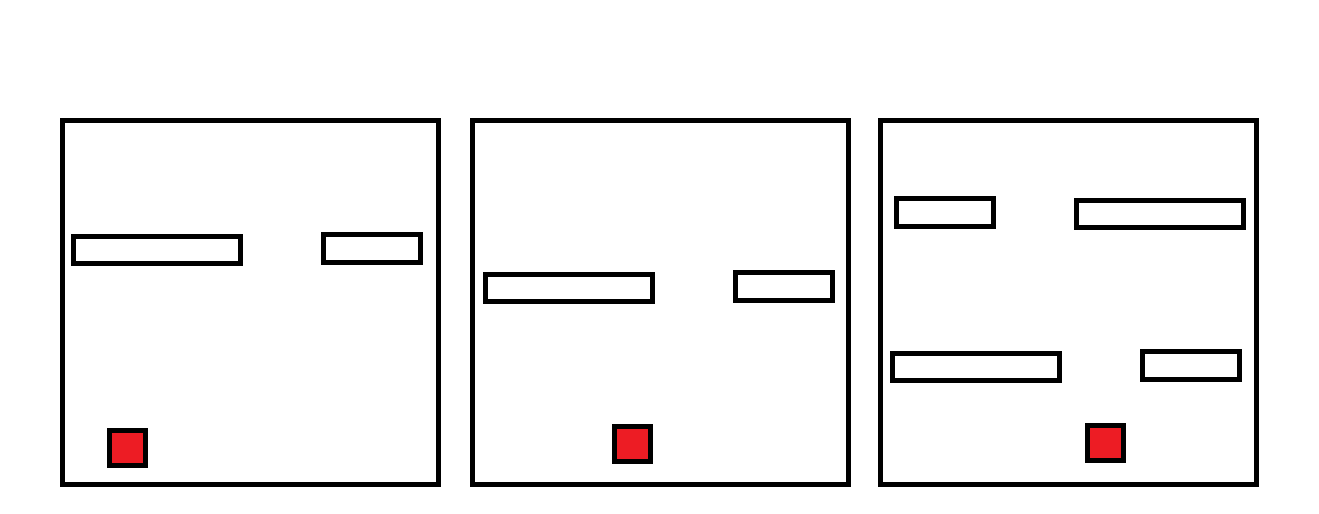
\includegraphics[width=4.5in]{display.png}
\caption{Time Progression of Gameplay}
\label{fig:disp}
\end{figure}
Our team plans to begin by ensuring the code is first developed and as bug-free as possible. We hope to be able to spend a lot of time debugging and optimizing the code. One of the last steps of our project will be dedicating time to ensure the form and function of the 3D-printed enclosure. We will do our best to stick to the parts list outlined in this report, but we have a few backup plans if things don't go according to plan. With this project, we hope to deliver a functional and fun experience for anyone interested in retro-style games who want to reduce their stress levels simultaneously.


\newpage
%\section{References}
\printbibliography[heading=subbibintoc]
%\bibliographystyle{plain}
%\bibliography{ref}

\end{document}
